\chapter{绪论}
自动驾驶技术作为人工智能和自动控制领域的前沿研究方向，近年来在学术界和工业界都引起了广泛关注。无人赛车作为一个极具挑战性的应用场景，不仅能够推动自动驾驶技术的发展，还能为实现高阶完全自动驾驶提供重要的技术积累和实践经验。本文将围绕无人赛车的运动控制与导航问题展开研究，旨在提升车辆在高速竞速环境中的安全性、稳定性和性能。本章首先介绍自动驾驶技术的发展背景和无人赛车的研究意义，然后综述和分析了无人赛车的运动控制与导航方法，最后概述本文的主要研究内容和组织结构。
\section{研究背景}
\subsection{自动驾驶行业背景与技术发展}
自动驾驶是指车辆在尽量少或无需人类驾驶员直接干预的情况下，依靠车载传感器、计算平台与智能算法完成环境感知、决策规划和运动控制等驾驶任务的技术体系\cite{pendleton2017perception}。从本质上看，自动驾驶是人工智能、控制科学与交通工程在复杂真实场景中的综合应用。其研究具有显著的现实意义与社会价值：一方面，道路交通事故中绝大多数源于人为失误，自动驾驶有望通过稳定、可重复的算法决策显著降低事故率\cite{fagnant2015preparing}；另一方面，自动驾驶可提升道路通行效率，减少拥堵和能耗，并为物流运输、共享出行和智慧城市提供关键技术支撑\cite{olayode2023systematic}。此外，在老龄化加剧和劳动力成本上升的背景下，自动驾驶被视为未来交通系统实现安全性、效率与可持续性协同提升的重要路径，因此成为学术界与工业界高度关注的前沿方向。

为了系统刻画车辆自动化能力，国际上通常采用分级标准对自动驾驶自主水平进行划分，其中最具代表性的是由国际汽车工程师学会提出的六级自动驾驶分级体系（L0–L5）\cite{J3016_202104}。L0–L2阶段以驾驶辅助为主，系统只能在特定工况下提供部分纵向或横向控制\cite{xu2017correctness}，驾驶责任仍主要由人类承担；L3阶段开始引入“有条件自动驾驶”，车辆在限定场景内可独立完成驾驶任务，但仍需要驾驶员在系统请求时接管\cite{morales2020automated}；L4阶段实现高度自动驾驶，车辆在设计运行域内可无需人工干预完成行驶\cite{scanlon2021waymo}；L5则代表完全自动驾驶，车辆在所有道路和环境条件下均可独立运行\cite{khan2022level}。该分级体系清晰反映了从“辅助”到“替代”的演进路径，也揭示了自动驾驶在安全性、责任划分和系统可靠性方面逐级提升的技术与工程挑战。

自动驾驶经历了从规则驱动到数据驱动、再到多模态融合的演进过程。早期研究主要依赖基于物理模型和人工规则的方法，通过明确的感知、规划与控制模块实现车辆在结构化环境中的自动行驶\cite{pendleton2017perception}。这一阶段强调系统可解释性和稳定性，但在复杂交通场景下对环境变化的适应能力有限\cite{yurtsever2020survey}。随着计算能力的提升和传感器成本的下降，多传感器融合技术迅速发展，摄像头、毫米波雷达与激光雷达相互补充，使车辆能够在动态、复杂环境中获得更全面的感知信息。同时，高精地图与高精定位技术的引入，显著提升了环境建模精度，为精细化路径规划提供了基础\cite{elghazaly2023high}。近年来，强化学习、模仿学习等数据驱动方法在自动驾驶领域取得了突破性进展，这类方法通过神经网络直接从传感器数据映射到控制指令，简化了传统模块化架构，提升了系统的适应性和泛化能力\cite{bojarski2016end, chitta2022transfuser, chen2024end}。强化学习使车辆能够通过与环境交互不断优化决策策略，实现复杂任务的自主学习\cite{kiran2021deep}；而模仿学习结合专家驾驶数据，提升了自动驾驶系统在实际道路条件下的表现\cite{grigorescu2020survey}。当前，自动驾驶技术正朝着多范式融合方向发展，将基于模型的方法与数据驱动方法相结合，以兼顾系统的可解释性与适应性，推动自动驾驶向更高水平迈进。
\subsection{无人赛车的运动控制与导航问题}
赛车作为一种高速下的极限运动，对自动驾驶车辆性能、环境感知、运动规划与跟踪控制策略提出了极高的标准和挑战\cite{betz2023tum}。与传统赛车运动非常类似，无人赛车同样提供了在具有挑战性的环境下开发和验证自动驾驶技术的条件，并促进这些先进技术在民用与商用车辆领域的部署应用\cite{betz2022autonomous}。无人赛车提供了一个独特的机会来测试自动驾驶系统的各个组成模块，如冗余感知、故障检测、运动规划及在高风险环境下的跟踪控制\cite{kabzan2020amz}。与赛车手参与下的赛车运动有所不同，无人赛车赛事能够在封闭环境内测试系统，降低人员伤害的风险。目前开展的无人赛车赛事主要有：DARPA自动驾驶挑战赛\cite{rouff2007introduction}、Roborace\cite{betz2019software}和Formula Student Driverless\cite{kabzan2020amz}等，如图\ref{fig:racing-games}所示。这些赛事为无人赛车的研发提供了宝贵的平台，推动了自动驾驶技术的进步。
\begin{figure}[ht]
    \centering
    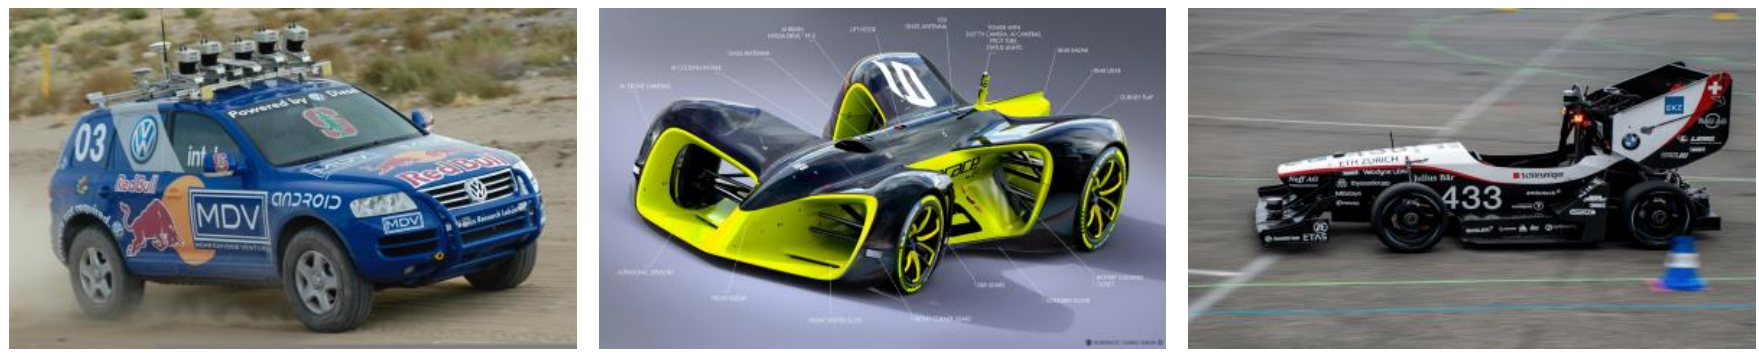
\includegraphics[width=1.0\linewidth]{figure/chapter1/racing-games.png}
    \caption{无人赛车赛事}
    \label{fig:racing-games}
\end{figure}

虽然公开道路上的自动驾驶车辆在大部分时间内主要运行在附着条件良好、机动平稳线性的工况下\cite{rajamani2006vehicle}，但为了实现完全自动驾驶赛车，一个关键问题是：车辆在接近动态极限以及道路附着极限时，能否以安全、稳定、高效的方式完成竞速任务\cite{talvala2011pushing}。因此，研究赛车运动控制与导航技术能驱动自动驾驶的创新迭代，并显著提升系统安全性能。该研究有助于自动驾驶技术的普及应用，对实现高阶完全自动驾驶具有重要意义。

竞速任务有两个评价指标：完成竞速任务的时间以及安全无碰撞的概率；因此，如何平衡这两个指标是赛车控制的关键问题\cite{liniger2015optimization}。车辆在高速行驶时，轮胎的摩擦力有可能达到饱和，产生横向位移，这就是所谓的“漂移”现象\cite{hindiyeh2013dynamics}。剧烈的漂移动作导致车辆的动力学模型难以准确估计，轮胎与路面的接触带来了极大的不确定性，给车辆的精准控制增加了挑战性\cite{goh2024beyond}。但是，如果能稳定控制像漂移这样高速运动的行为，那么车辆的运动性能可以显著提升，并在紧急避障、车辆打滑等状态下提高安全系数。然而，高速运动车辆的控制面临着多种挑战，例如车辆动力学响应的非线性特性、状态量的高度耦合等\cite{rajamani2006vehicle}；此外，车辆在高速行驶过程中，环境感知和路径规划的实时性和准确性也对运动控制提出了更高的要求\cite{kabzan2020amz, heilmeier2020minimum, drews2019vision}。近年来，随着计算能力的提升和传感器技术的发展，越来越多的研究开始关注如何在高速运动状态下实现对车辆的精准控制与导航。现有的研究主要集中在基于模型的方法和基于深度学习的方法两大类。

\section{高速运动控制与导航研究现状}
\subsection{基于模型的方法}
\subsubsection{基于图搜索的方法}
图搜索算法可以分为深度优先搜索、广度优先搜索和最佳优先搜索。深度 优先搜索算法尽可能深入、快速地构建搜索树，直到找到合适的路径。而广度优先搜索算法中的搜索树则是通过尽可能广泛和快速地扩展节点来实现。最佳优先搜索算法为搜索树中的每个节点和边添加一个数值准则（值或成本）。

Dijkstra 算法\cite{dijkstra2022note}是基于最佳优先搜索寻找最短路径的算法之一。算法通过计算图中节点之间的距离不断选取距离源节点最近的节点，直到找到起点和目的地之间的最短距离。Dijkstra 算法的解一定是最优的，然而其扩展节点过多，十分消耗内存和计算时间，不适合在线更新计算。

A*算法\cite{hart1968formal}是基于启发式函数进行快速节点搜索的图搜索算法，是Dijkstra算法的拓展。A*算法最重要的设计是代价函数的确定，它定义了节点的权重，决定了哪些节点将被访问。该算法虽然求解速度比Dijkstra算法快很多，但在复杂场景下仍然不满足实时路径规划需求。移动机器人领域有很多基于A*算法的改进，如Dynamic A*(D*)、Field D*、Theta*等。Ziegler等人实现了基于Voronoi图的A*算法，用于非结构化空间和停车场的运动规划\cite{ziegler2008navigating}。另外，在2007年HybridA*算法第一次被用于DARPA城市挑战赛中\cite{dolgov2008practical}，文中对A*算法的改进使求得的解可以被用于具有非完整约束的车辆上。

基于图搜索的算法的优点是可以找到全局最优解，且易于实现。然而，这类算法通常需要对环境进行离散化处理，导致计算复杂度较高，难以满足实时性要求。此外，图搜索算法在处理动态环境时表现不佳，因为每次环境变化都可能需要重新构建图，从而增加了计算负担。
\subsubsection{基于采样的方法}
与基于图搜索的方法相比，基于采样的路径规划算法不需要显式构建整个配置空间和边界。该方法对配置空间或状态空间进行随机采样，寻找其内部的时空连通性。该方法的缺点是求得的解不能保证是最优的。在机器人学中最常用的方法是RRT算法。

RRT(Rapidly-Exploring Random Tree)算法\cite{lavalle1998rapidly}，是一种适用于在线路径规划的基于采样的算法。它通过在导航区域执行随机搜索，并构建搜索树实现快速规划。然而，RRT 在整个空间上进行采样的效率有待提高。Karaman等人提出了RRT*算法\cite{karaman2011sampling}，该算法在RRT的基础上引入了路径优化的步骤，通过重新连接节点来不断改进路径质量，从而实现渐近最优性。RRT*算法在采样过程中考虑了路径的成本，使得生成的路径不仅可行，而且趋近于最优路径。针对RRT*算法生成的路径不平滑的问题，有人提出了可以生成符合机器人动力学约束的路径的算法：Kinodynamic-RRT*\cite{webb2013kinodynamic}，该算法改进了RRT*算法的 Steer() 函数，使得节点之间的路径更加平滑。另外，RRT*算法在找到一条从起点到终点的路径之后，会持续对路径进行优化，而该优化过程依赖于整个地图中的新采样点，因此计算效率相对较低。Informed RRT*算法\cite{gammell2014informed}将优化的范围限制在路径周围的椭圆内，因此大大提高了效率。然而，RRT及其变种算法在高维空间中的性能仍然有限，且生成的路径可能不够平滑，需要后续处理；另外，对于高速运动中轮胎动力学等复杂的车辆动力学模型，RRT算法难以获得理想的效果。
\subsubsection{基于数值优化的方法}
运动控制问题可以被形式化为一个最优控制问题（Optimal Control Problem，简称OCP），其目标是通过优化某个性能指标（如时间、能量消耗等）来确定车辆的控制输入，从而实现对车辆的精确控制\cite{lewis2012optimal}。最优控制问题通常可以表示为如下形式：
\begin{equation}
\begin{aligned}
 \min_{u(\cdot)}\quad & J=\Phi(x(t_f),t_f)+\int_{t_0}^{t_f}L(x(t),u(t),t)dt \\
 \text{s.t.}\quad & \dot{x}(t)=f(x(t),u(t),t),\ t\in[t_0,t_f] \\
 & x(t_0)=x_0 \\
 & x(t)\in\mathcal{X},\ u(t)\in\mathcal{U} \\
 & g(x(t),u(t),t)\leq0
\end{aligned}
\label{equ:ocp}
\end{equation}
其中，$x(t)$表示车辆的状态变量，$u(t)$表示控制输入，$J$表示性能指标，$\Phi$表示终端成本，$L$表示运行成本，$f$表示车辆的动力学模型，$g$表示约束条件，$\mathcal{X}$和$\mathcal{U}$分别表示状态空间和控制输入空间。求解最优控制问题的方法大体可分为“分层规划+跟踪”和“规划控制一体化”两类。

Heilmeier等人提出了一种层级规划-控制框架，用于无人赛车的路径规划与跟踪控制\cite{heilmeier2020minimum}。该方法首先通过预先建图与轨迹规划的方法生成一条最小化曲率的竞速轨迹，然后利用下层控制器进行轨迹跟踪。然而，这种层级框架依赖于高精度地图，且轨迹规划与跟踪控制是分离进行的，跟踪误差容易造成危险的碰撞行为。规划控制一体化的方法通常使用模型预测控制（Model Predictive Control，简称MPC）来实现竞速运动控制。MPC在有限时域内通过模型预测和迭代优化的方法计算控制量的最优解，它的数学形式支持各种约束条件（例如安全避障约束和状态量范围约束）以及多目标优化（例如最小化时间和最小化轨迹平滑度）\cite{MOTO201303005}。在无人赛车竞速的场景中，MPC的核心是构建车辆的动力学模型以及时间最优控制问题：过于简化的模型不能准确描述车辆动力学，会降低预测性能；过于复杂的动力学使得优化问题难以求解，不能满足实时性\cite{dixit2019trajectory}；并且，时间最优控制问题非凸性强，容易陷入局部最优\cite{sedlacek2021minimum}。现有基于MPC的方法有如下几类：Liniger等人提出了一种基于模型预测轮廓控制（Model Predictive Contouring Control，简称MPCC）的方法，用于无人赛车的运动规划与控制\cite{liniger2015optimization}。该方法通过在线求解一个有限时间的最优控制问题，生成车辆的参考轨迹和控制输入，从而实现对车辆的精准控制。该方法考虑了车辆的动力学约束和环境约束，能够在复杂的赛道环境中实现高效的运动规划与控制。然而，轮胎与路面的摩擦具有不确定性，模型的不准确容易使控制器的稳定性失效。为了应对极限工况下轮胎摩擦的不确定性，Kabzan等人提出了一种基于学习的模型预测控制方法（Learning-Based Model Predictive Control，简称LMPC）\cite{kabzan2019learning}，通过在线更新车辆动力学模型，提高了控制器在极限工况下的鲁棒性和性能。然而，该方法依赖于大量的训练数据，且在线学习过程可能导致计算开销较大，影响实时性。Rosolia等人提出了相似的迭代学习模型预测控制，通过迭代学习Q函数来实现优异的控制效果\cite{rosolia2019learning}。然而，在迭代优化的前期控制器无法保证安全性和稳定性，限制了其在实物系统中的应用。因此，如何平衡MPC在极限工况下的稳定性、安全性和实时性仍然是一个亟待解决的问题。

\subsection{基于深度学习的方法}
基于深度学习的方法，例如模仿学习和强化学习，可以通过神经网络拟合函数的方式，直接将传感器观测到的状态映射到控制量，用参数化策略克服传统模块化和基于模型的方法的局限性。基于学习的方法的一个主要优势是它们不需要对车辆及其环境有太多的先验知识。通过大量的数据训练，深度神经网络可以自动学习复杂的非线性关系，从而实现对车辆运动的精准控制。此外，基于深度学习的方法具有较强的适应性，能够在不同的环境和条件下表现出良好的性能。

\begin{figure}[ht]
    \centering
    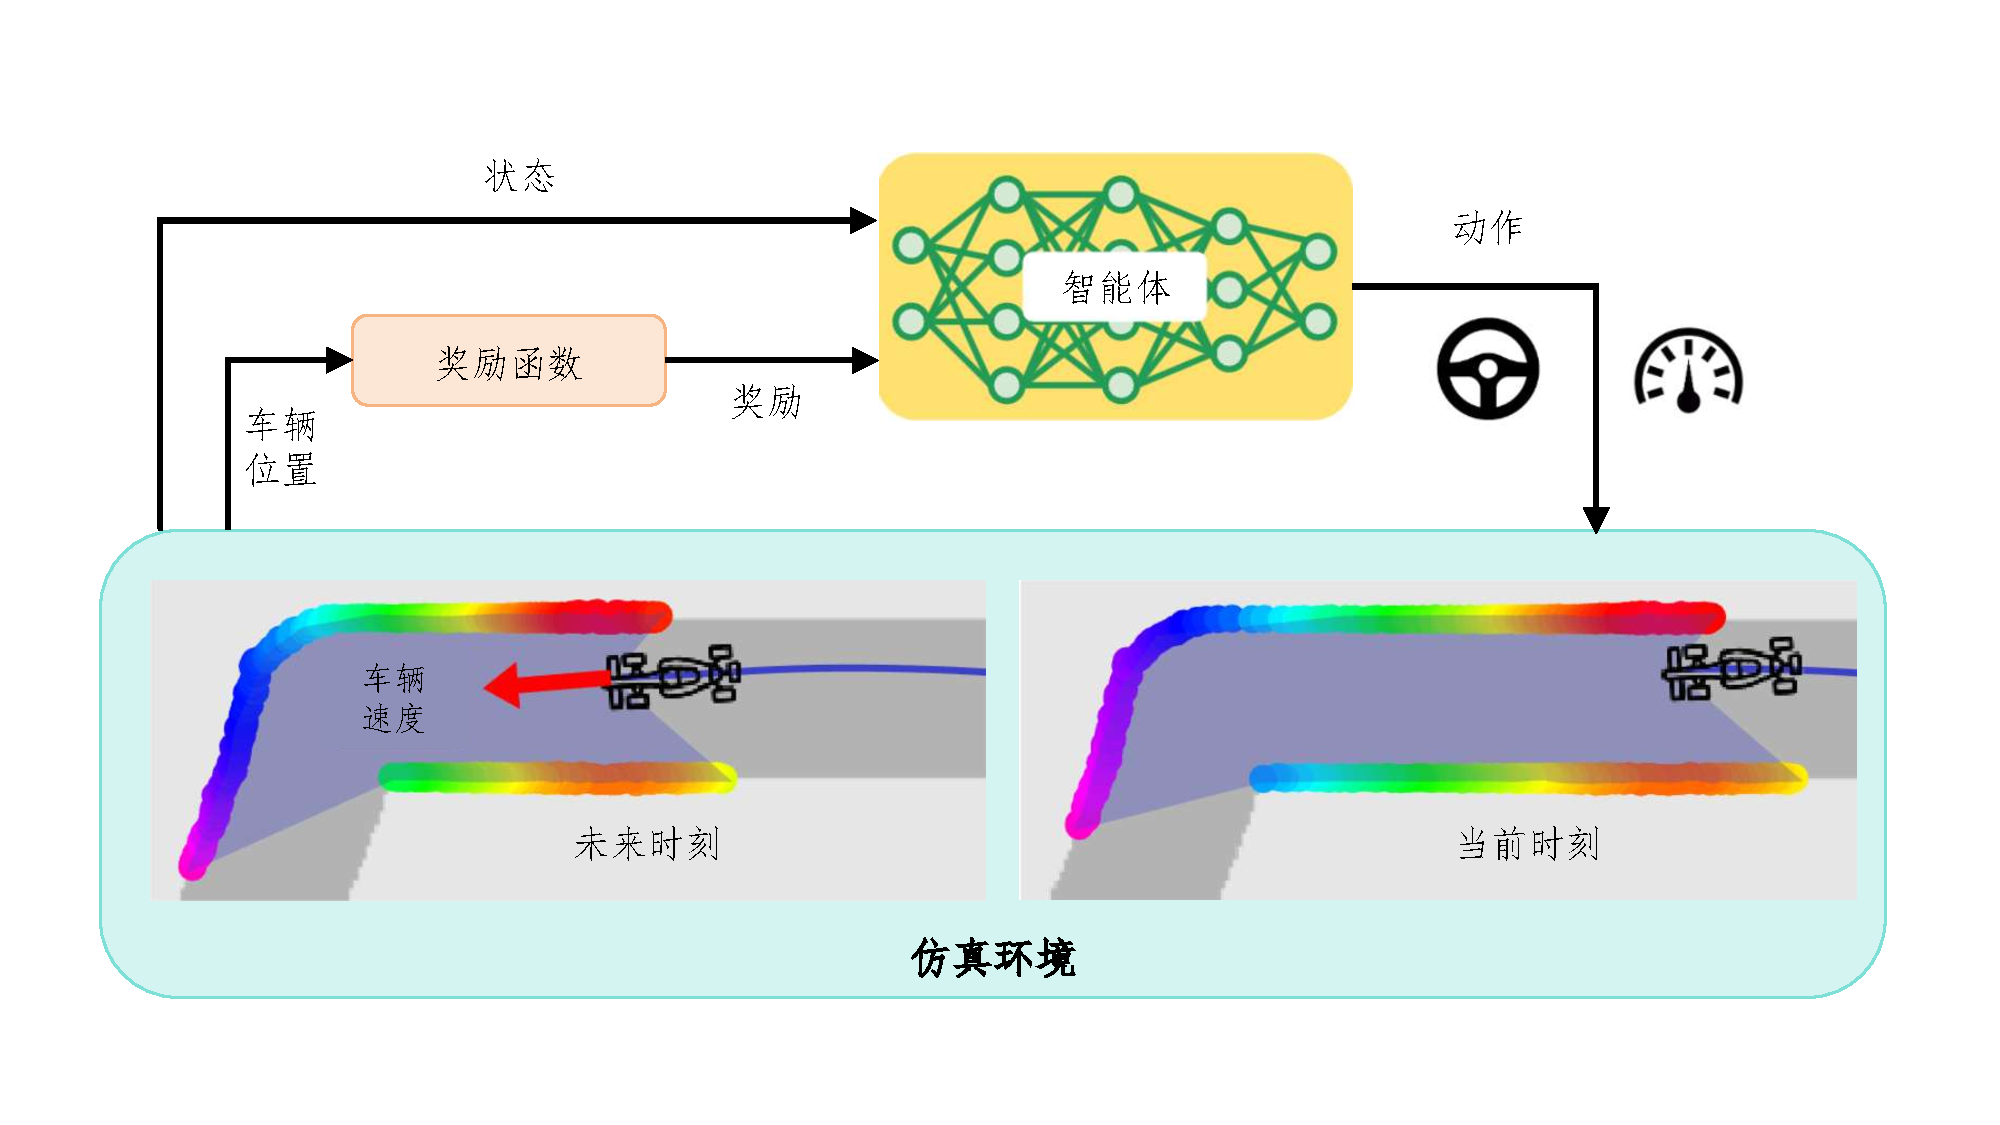
\includegraphics[width=0.9\linewidth]{figure/chapter1/rl.pdf}
    \caption{强化学习用于赛车环境的示意图}
    \label{fig:reinforcement-learning}
\end{figure}
强化学习（Reinforcement Learning，简称RL）通过智能体与动态环境之间的持续交互来学习控制策略。对于无人赛车任务而言，智能体在每个时刻根据车载传感器提供的观测信息，例如激光雷达、车辆速度、航向角以及相对赛道位置等，输出转向、油门和制动等低层控制指令，如图\ref{fig:reinforcement-learning}所示。强化学习通常使用演员-评论家（Actor-Critic）架构，即评论家（Critic）网络估计状态或状态动作对的价值函数，演员（Actor）网络根据当前观测输出动作分布或确定性控制量。已有研究表明，强化学习在端到端无人赛车控制、竞速决策以及复杂博弈式驾驶中均表现出较强潜力\cite{perot2017end, wurman2022outracing}。强化学习分为无模型的强化学习和基于模型的强化学习。无模型强化学习不显式学习系统动力学，而是直接利用采样得到的交互轨迹来优化参数化策略或价值函数。Fuchs等人使用软演员-批评家（Soft Actor-Critic，简称SAC）算法在高保真Gran Turismo Sport仿真环境中训练无人赛车控制策略，实现了超过人类玩家的竞速表现\cite{fuchs2021super}。Evans等人提出了用于高性能无人赛车的轨迹辅助学习（Trajectory-Aided Learning，简称TAL），将传统赛车规划方法和深度强化学习相结合，从而利用先验轨迹知识缩短训练时间并提升高速场景下的完成率与稳定性\cite{evans2023high}。然而，无模型强化学习的主要问题在于样本效率较低，训练过程往往需要长时间随机探索。相比之下，基于模型的强化学习通过显式学习环境动力学模型，可以在想象的轨迹上更新策略，通常能够提高样本的利用效率。Hafner等人引入了基于模型的强化学习算法Dreamer来学习潜在空间中动力学模型，并在潜在空间中进行想象交互来优化策略\cite{hafner2020mastering}。Brunnbauer等人将Dreamer算法引入无人赛车任务，证明了潜在想象机制能够提高赛车策略的泛化能力，并支持从仿真到真实平台的零样本迁移\cite{brunnbauer2022latent}。然而，基于模型的强化学习性能高度依赖所学动力学模型的精度，一旦模型在长时域预测中出现偏差，误差便会在轨迹中逐步累积，导致策略的泛化性能下降\cite{janner2019trust}。

模仿学习（Imitation Learning, IL）也是无人赛车中常用的一类端到端策略学习方法。与强化学习不同，模仿学习主要通过监督学习的方式直接拟合专家策略，将专家在给定观测下采取的动作作为标签，训练从传感器输入到控制输出之间的映射关系。因此，模仿学习不需要显式定义复杂的奖励函数，也避免了强化学习中高成本的在线探索过程，使其在训练效率、实现复杂度和工程落地性方面具有明显优势\cite{mehta2018learning, weiss2020deepracing}。Bojarski等人提出了端到端驾驶框架NVIDIA DAVE-2，通过卷积神经网络（Convolutional Neural Network，简称CNN）直接根据前向摄像头图像预测转向指令，并据此实现车辆的闭环控制\cite{bojarski2016end}。类似地，Pan等人利用专家示范数据训练策略网络，实现了敏捷驾驶和越野无人驾驶任务，表明模仿学习也能够扩展到高速、低附着和非结构化环境中的车辆控制问题\cite{pan2020imitation}。在赛车场景中，Weiss等人提出的 DeepRacing进一步展示了模仿学习在高性能竞速中的应用潜力\cite{weiss2020deepracing}。然而，模仿学习存在一个根本性问题，即训练数据分布与测试时策略接收的状态分布不一致。这种训练—测试分布不匹配是限制模仿学习鲁棒性的核心因素。Ross等人提出了用于在线模仿学习的数据集聚合（Dataset Aggregation，简称DAgger）来解决这个问题\cite{ross2011reduction}。然而，即使模仿学习算法克服了适应性的限制，但它们的性能仍取决于数据集的规模和质量，而且很难超过专家\cite{codevilla2018end}。

在实际赛车比赛中，人类驾驶员通常只能依赖车载局部传感信息进行决策，而无法直接访问完整环境信息。因此，从应用角度看，仅利用车载视觉和本体状态实现端到端自动驾驶赛车，具有更强的现实意义和部署价值。以往的研究大多依赖预先构建的高精度地图以及赛道边界信息，一旦赛道布局变化或感知条件恶化，其性能往往会显著下降。为了克服这一挑战，近年来出现了一些结合视觉感知和深度学习的方法。Jaritz等人提出了一种基于前向RGB图像的端到端深度强化学习赛车方法，利用A3C框架学习车辆控制策略\cite{jaritz2018end}。然而该方法无法持续生成安全竞速轨迹，在驾驶过程中可能出现危险的碰撞，并未系统解决高速运动控制中的安全性与稳定性问题。Cai等人提出了视觉驱动赛车的深度模仿强化学习方法（Deep Imitative Reinforcement Learning，简称DIRL），将模仿学习与强化学习相结合，在现实竞速比赛中显著提升了成功率\cite{cai2021vision}。然而，这类方法仍然存在性能受限的问题，即闭环执行时策略往往倾向于采取更保守的控制方式。因此，当训练过程中缺少足够的全局信息时，即使策略具备较好的可行性和鲁棒性，也未必能达到最优竞速性能；另外，高维视觉观测还会进一步放大强化学习的数据效率问题，高容量视觉编码器仅依赖稀疏奖励进行训练时样本效率很低，且容易导致训练不稳定与次优收敛\cite{yarats2021improving}。为了解决以上问题，Vasco等人提出了非对称的深度强化学习方法：评论家网络可以访问仿真中的全局信息，而演员网络只使用车载局部观测，在Gran Turismo Sport高保真赛车环境中实现了超越人类的表现\cite{vasco2024super}。然而，仿真与现实世界中动力学、视觉信息的差距会影响策略的实际控制效果\cite{peng2018sim}，该方法仅在仿真环境中测试，并未在有噪声的现实世界中测试其鲁棒性。因此，如何将仿真中学到的策略成功迁移到现实世界仍是一个亟待解决的问题。
\section{本文主要研究内容}
\subsection{研究内容与主要贡献}
根据上述研究背景与研究现状可知，高速无人赛车的运动控制与导航问题还存在以下挑战：在高速运动的条件下，车辆的动力学呈现高度的非线性特征，运动状态之间存在高度耦合，因此系统对模型误差、环境变化和感知不确定性高度敏感。同时，无人赛车的运动控制与导航还需要平衡竞速性能与安全性。此外，在未知复杂环境下，车辆需要依赖车载视觉等局部观测进行决策，这进一步增加了感知不确定性和控制难度。

围绕上述问题，本文按照“安全运动控制—视觉竞速—高速导航”的技术主线，系统开展了以下三个递进式的研究：首先，针对无人赛车在接近动态极限时的安全控制问题，本文建立了无人赛车动力学模型并进行了关键参数辨识，在此基础上将控制障碍函数与模型预测控制相结合，提出一种兼顾竞速性能与避障能力的安全运动控制方法。其次，针对无人赛车在未知赛道中基于深度视觉的竞速控制问题，本文提出了一种融合特权信息的教师—学生两阶段策略学习方法，通过强化学习训练教师策略，并借助知识蒸馏将高性能控制能力迁移到基于深度视觉的学生策略。最后，针对无人赛车在未知环境中的高速点到点导航问题，本文提出了一种基于视觉预测模型的导航方法，通过学习环境的时序演化规律并结合采样式模型预测控制，实现感知、预测与决策的导航框架。

围绕上述研究内容，本文的主要贡献如下：
\begin{enumerate}
    \item 针对无人赛车在接近动态极限时的安全控制问题，本文构建了能够描述极限工况下车辆运动行为的动力学模型，并通过系统辨识获得关键参数；在此基础上，提出基于控制障碍函数的安全竞速控制方法。该方法将安全约束显式嵌入模型预测控制框架，使得车辆在接近动态极限条件下仍能满足竞速的安全性要求。该方法在理论上保证系统的前向不变性，能够在保证安全性的同时兼顾车辆的动态性能，提升了高速竞速场景下的鲁棒性与安全性。
    \item 针对无人赛车在未知赛道中基于深度视觉的竞速控制问题，本文提出了一种教师—学生两阶段学习方法。为解决视觉强化学习中样本效率低和训练不稳定的问题，本文融合特权信息设计了教师策略训练机制，通过强化学习获得高性能参考策略；随后引入知识蒸馏方法，将教师策略的决策能力迁移至仅依赖视觉输入的学生策略。学生网络中融合了视觉变分自编码器和循环神经网络，用于消除图像噪声和部分可观性的影响，从而提升了策略的泛化能力和竞速性能。
    \item 针对无人赛车在未知环境中的高速点到点导航问题，本文引入了视觉预测模型，构建了包含感知—预测—控制的端到端导航框架。通过学习环境的演化规律，视觉预测模型可以预测未来的观测分布，并结合采样式模型预测控制进行决策优化，实现基于未来场景推演的控制策略。相较于仅基于当前观测的反应式控制，该方法能够显式考虑未来风险与可行轨迹空间，并优化较长的控制序列，从而在复杂环境中实现更稳定的导航表现，且具备更强的可解释性。
\end{enumerate}

\subsection{本文组织架构}
本文的组织架构如图\ref{fig:structure}所示，共分为五个章节：
\begin{figure}[ht]
    \centering
    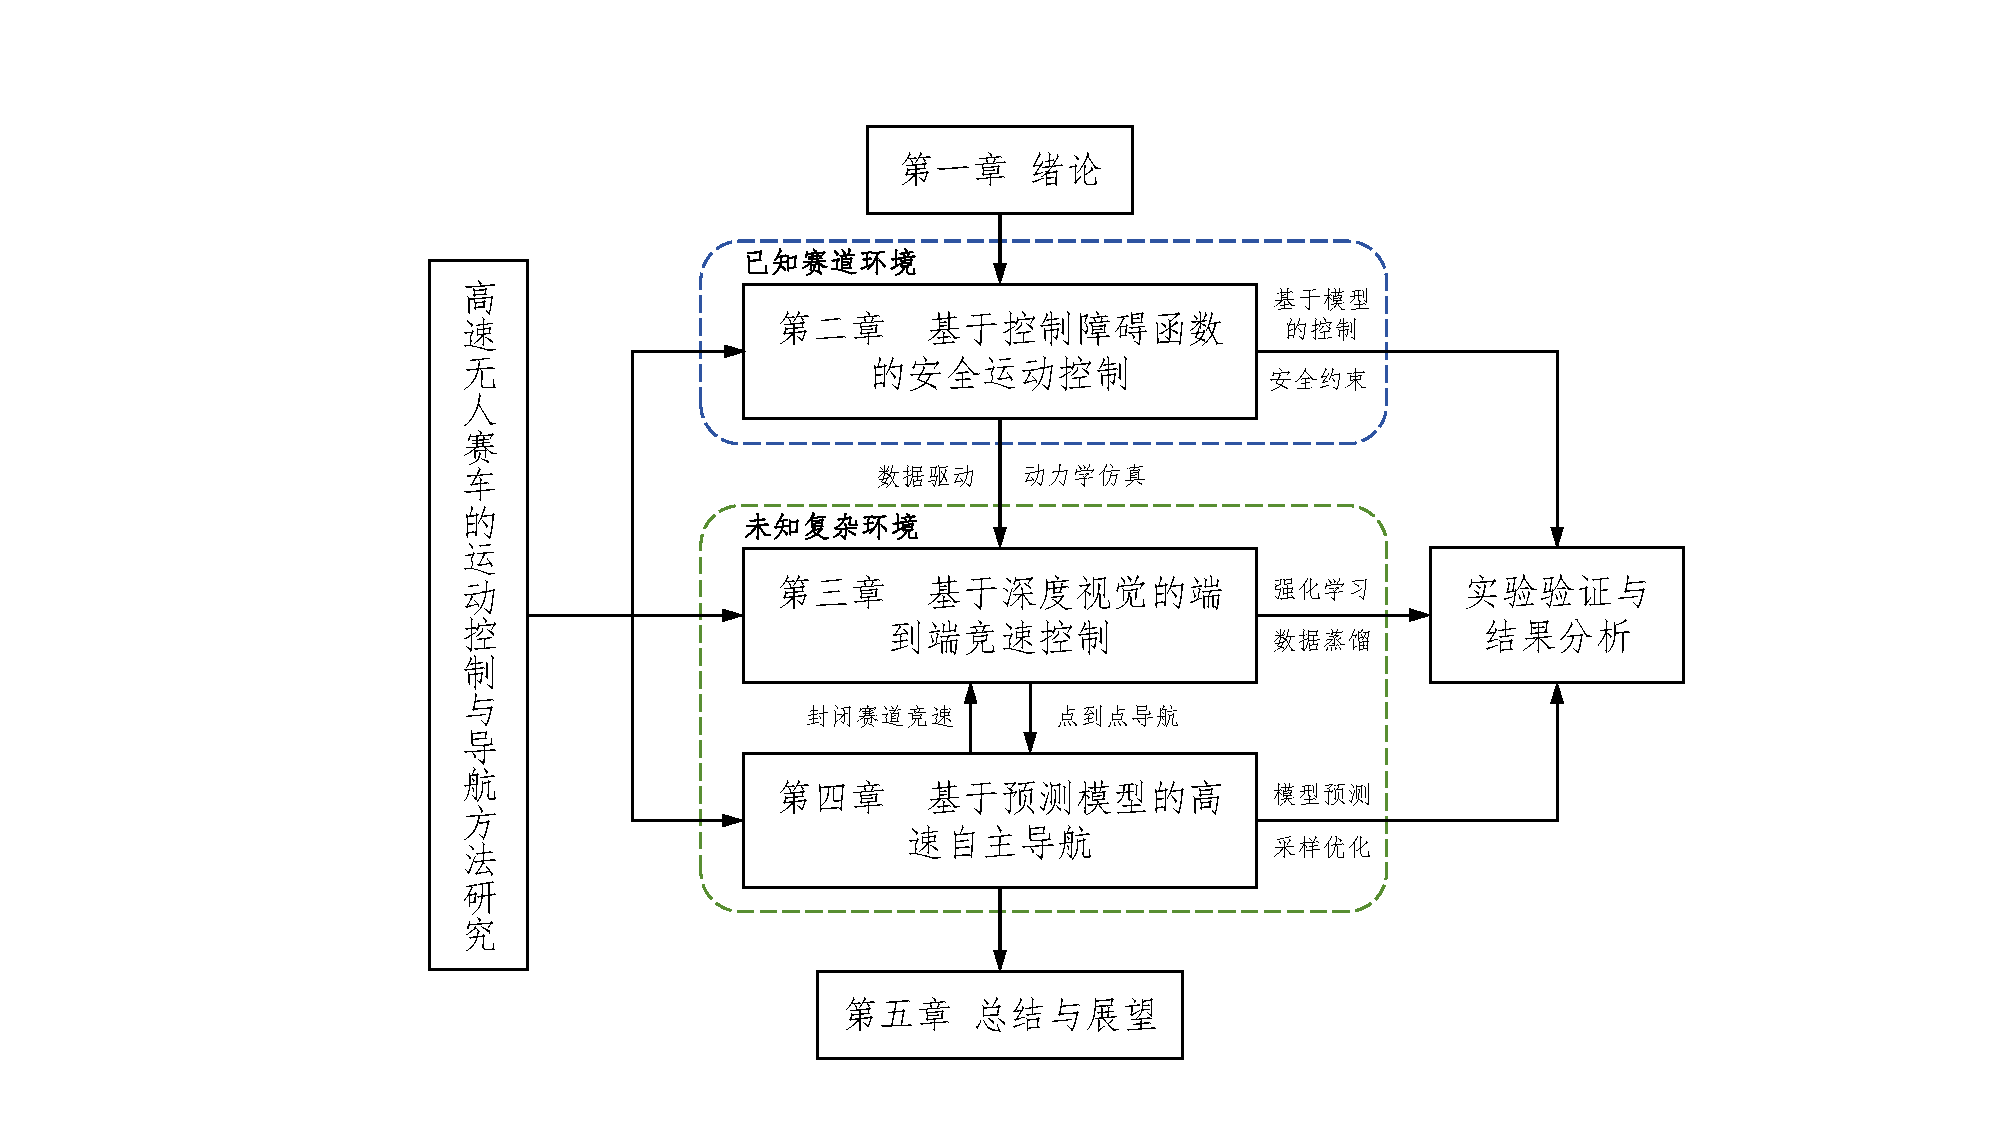
\includegraphics[width=0.8\linewidth]{figure/chapter1/structure.pdf}
    \caption{论文组织架构图}
    \label{fig:structure}
\end{figure}

第一章：绪论。本章首先介绍了自动驾驶的行业背景和发展历程，阐述了无人赛车对于推动智能驾驶技术发展的重要意义，并分析了高速运动控制面临的挑战。随后，系统综述了无人赛车运动控制与导航领域的研究现状，涵盖了基于模型的方法和基于深度学习的方法，比较不同技术路线在安全性、实时性与泛化能力等方面的优势与局限。最后，明确了本文的主要研究内容和贡献，并概述了论文的组织结构。

第二章：基于控制障碍函数的安全运动控制。本章首先建立车辆动力学模型，并通过参数辨识获得模型参数，为后续控制策略设计提供基础。随后介绍控制障碍函数的基本理论，并将其与模型预测控制框架相结合，构建兼顾性能优化与安全约束的运动控制策略，使车辆在接近动态极限条件下仍能满足赛道边界、动态障碍物等安全性要求。最后通过仿真实验与实车实验对所提出方法进行验证，并从竞速性能、控制稳定性及安全性等方面对结果进行分析。

第三章：基于深度视觉的端到端竞速控制。本章提出了一种两阶段的端到端运动策略学习框架。首先构建融合特权信息的教师策略训练机制，通过强化学习使其在可获得完整环境信息条件下学习高性能控制行为；随后引入知识蒸馏方法，将教师策略的决策能力迁移至仅依赖视觉输入的端到端学生网络。学生网络中融合了视觉变分自编码器和循环神经网络，用于消除深度图像中噪声和部分可观性的影响。最后通过竞速性能对比实验、消融实验以及仿真到实车迁移实验，对所提出方法的泛化能力与实际应用效果进行系统评估。

第四章：基于预测模型的高速自主导航。本章首先对视觉导航任务进行问题建模，分析在复杂环境中仅依赖当前观测进行决策所面临的局限性。随后引入了视觉预测模型，通过学习环境的时序变化规律，实现对未来观测状态的预测，并给出相应的训练方法。同时结合基于采样的模型预测控制方法，通过采样的方法减少模型的强非线性对策略优化的影响，构建了一个感知—预测—控制一体化的端到端导航框架。最后通过仿真实验对导航性能进行系统验证，并通过对比实验与消融实验分析预测模型对控制性能提升的作用。

第五章：总结与展望。本章对论文的研究工作进行归纳，总结本文在安全控制、端到端竞速以及高速自主导航等方面取得的主要研究成果，突出了本文的研究价值及创新性。同时，本章分析了研究的局限性和改进空间，对未来自动驾驶运动控制的发展方向进行展望。